\part{User Manual}\label{part2}
\noindent
It is assumed that the reader has studied the MCLab Handbook before using CSE1, and has knowledge about Lab equipment, procedures and Safety precautions. In addition, keep the following in mind when using CSE1:
\begin{description}
	\item [{Water~damage:}] CSE1 is not waterproof and has excessive thrust capability which can inflict large roll angles. The risk of water on deck is reduced through thrust limitation and HIL testing before application of new control algorithms. 
	\item [{Propeller~dry~running:}] BT must only be run in water. Before removing the vessel from the water, the control system must be stopped and the VeriStand project undeployed.
	\item [{Loss~of~laptop~control:}] Wireless network instability may result in loss of connection between the laptop user interface and the cRIO. In this event, fall back to manual thruster control, by pushing 
\includegraphics[scale=0.4]{fig/sixaxis_triangle} on the Sixaxis. Alternatively, press 
\includegraphics[scale=0.4]{fig/sixaxis_circle} to stop the vessel.
	\item [{Total~loss~of~control:}] Pull CSE1 with a boat hook, and keep the vessel in water while disconnecting batteries.
\end{description}
\chapter{Launching}
\textit{Describe hardware preparations, establishing connection, building and including simulink model, uploading code to vessel}

\section{Vessel and lab preparations}
The gear in the bow thruster is lubricated with water, and thus it is IMPORTANT that the vessel is always launched in the basin when starting up/deploying the code. Hence, do as follows: 
\begin{enumerate}
	\item Place the vessel in the basin
	\item Check that the 1kg weight in the bow is placed at its position, in front of the cRIO box. 
	\item Place the 12V 12Ah battery(marked CSE1) in its dedicated position. Connect red/positive first, then black/negative.  
	\item Once the Bluetooth dongle (connected to the RPi) starts blinking(blue light with frequency approx. 1 Hz), press the PS-button on the sixaxis controller. On the controller, indicator 1 lights continuously red when successfully connected. 
	\item Place the vessel inside the region of sight for Qualisys(check on the computer that the 4 reflectors are visible). Align the vessel with 0 degrees heading in the basin frame, i.e. with the bow pointing towards the command center. 
	\item On the Qualisys computer(labeled \textit{QTM Surface}), start Qualisys Track Manager. In the upper left corner, press 
\includegraphics{fig/new_measurement.png} to start new measurement, then press 
\includegraphics{fig/project_options.png} to open the setting. In the left pane, navigate to 6DOF Tracking. Remove existing bodies and then press Aqcuire Body(verify CSE1 has 0\degree heading when pressing). Qualisys should find the 4 markers on the vessel(check 3D window to verify the body. If extra markers/points are found, remove them from the body in settings). Press Translate, and define CO from the highest marker(i.e. the one with lowest z-coordinate, typically -150mm) such that it has the body coordinates (x,y,z)=(550,0,-500)[mm].  See Figure \ref{fig:QTM_window} for illustration, or see the MCLab Handbook for further explanation and debugging. 
	\item Go to 3D visualization window, and verify that the body is defined correct (body frame position and orientation relative the 4 markers).
\end{enumerate}
\begin{figure}[htb!]
	\centering
	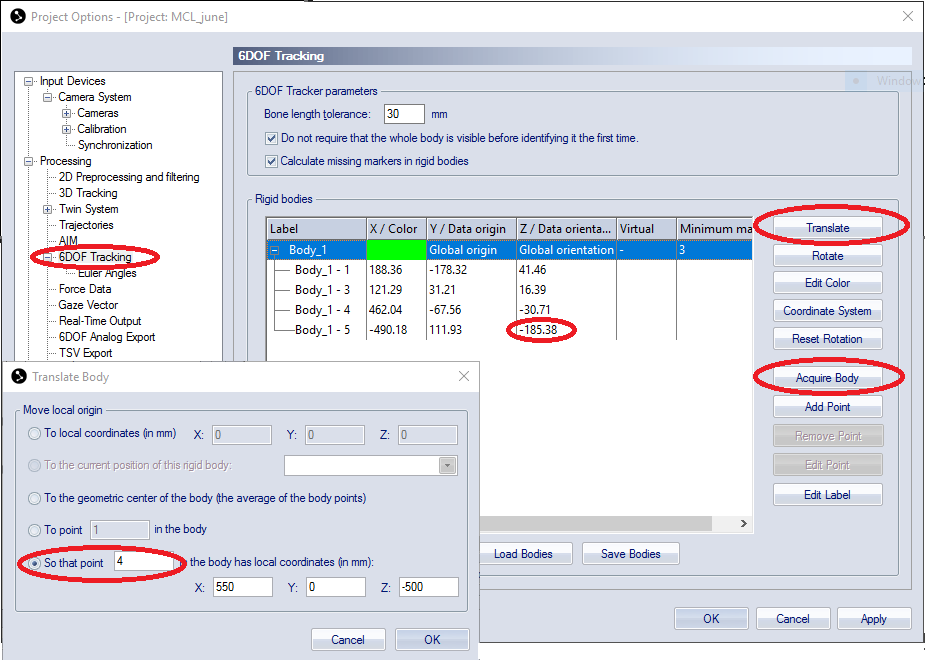
\includegraphics[scale=0.5]{fig/QTM_window.png}
	\caption{QTM window}
	\label{fig:QTM_window}
\end{figure}
CSE1 and the lab is now set up for experiments. However, before continuing to controlling the vessel, make sure the vessel does not take in water(there have been some issues with leakage in the hull opening around the bow thruster...)
\section{Updating custom control system}
See the MC-Lab Handbook for instructions on how to update and include your customized control system in the VeriStand project. Once you have completed the steps described there, continue here with uploading the code to the vessel. 
\section{Upload VeriStand project to the vessel}
With the hardware set up and ready, continue to preparing the software. 
\begin{enumerate}
	\item Make sure the computer is connected to the MCLab network(either by Ethernet cable or the WiFi). 
	\item Check the communication between the laptop and CSE1. Open command prompt(cmd.exe), write the following: \texttt{ping 192.168.0.75}. Make sure the command returns 0\% loss.
	\item Open the VeriStand project (\textit{CSE1.nivsproj}). Press the deploy button(see Figure \ref{fig:project_explorer}) or F6. The project is now uploading to the cRIO on board CSE1. If deployment is not successful, make sure the sixaxis controller is still connected to the RPi, and that the vessel body is shown in Qualisys. Try deploying again. If it still does not work, try restarting the vessel(either disconnecting the battery and connecting it again, or restart the cRIO in NI MAX). Also check that the Qualisys computer is connected to MCLab(\texttt{ping 192.168.0.10}). 
	\item When successfully deployed, open the Workspace (\textit{CSE1.nivsscreen}). The code is now running on the cRIO, continue to the next Chapter for instructions on operating the vessel. 
\end{enumerate}
\begin{figure}[htb!]
	\centering
	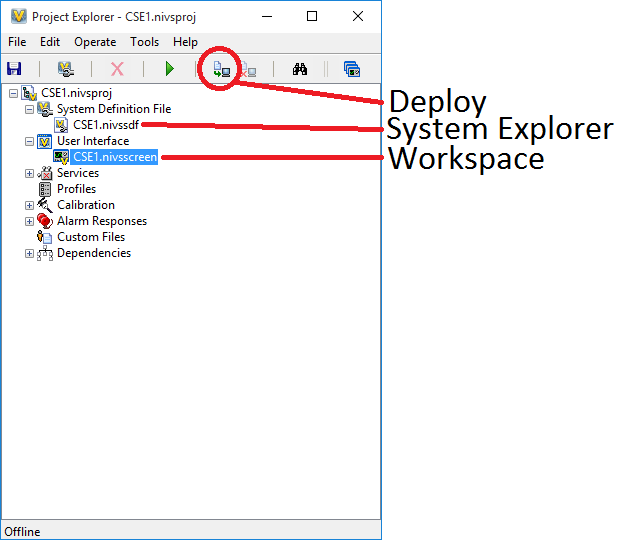
\includegraphics[scale=0.8]{fig/project_explorer.png}
	\caption{User interface in VeriStand Project Explorer}
	\label{fig:project_explorer}
\end{figure}
\chapter{Operation}
After successfully deploying the VeriStand project, you control the vessel with the sixaxis-controller and/or the laptop. Use the sixaxis-controller to switch between the different operation modes:
\begin{itemize}
	\item 
\includegraphics[scale=0.5]{fig/sixaxis_triangle.png} - ctrl\_sixaxis2thruster
	\item 
\includegraphics[scale=0.5]{fig/sixaxis_square.png} - ctrl\_custom
	\item 
\includegraphics[scale=0.5]{fig/sixaxis_cross.png} - ctrl\_DP
	\item 
\includegraphics[scale=0.5]{fig/sixaxis_circle.png} - STOP
\end{itemize}
Data logging can be done in two ways, as described in the MC-Lab Handbook. 
\section{Workspace}
On the laptop, use the Workspace to monitor the different variables. There are 3 screens, one for each operating mode: 
\paragraph{ctrl\_sixaxis2thruster}
\begin{figure}[htb!]
	\centering
	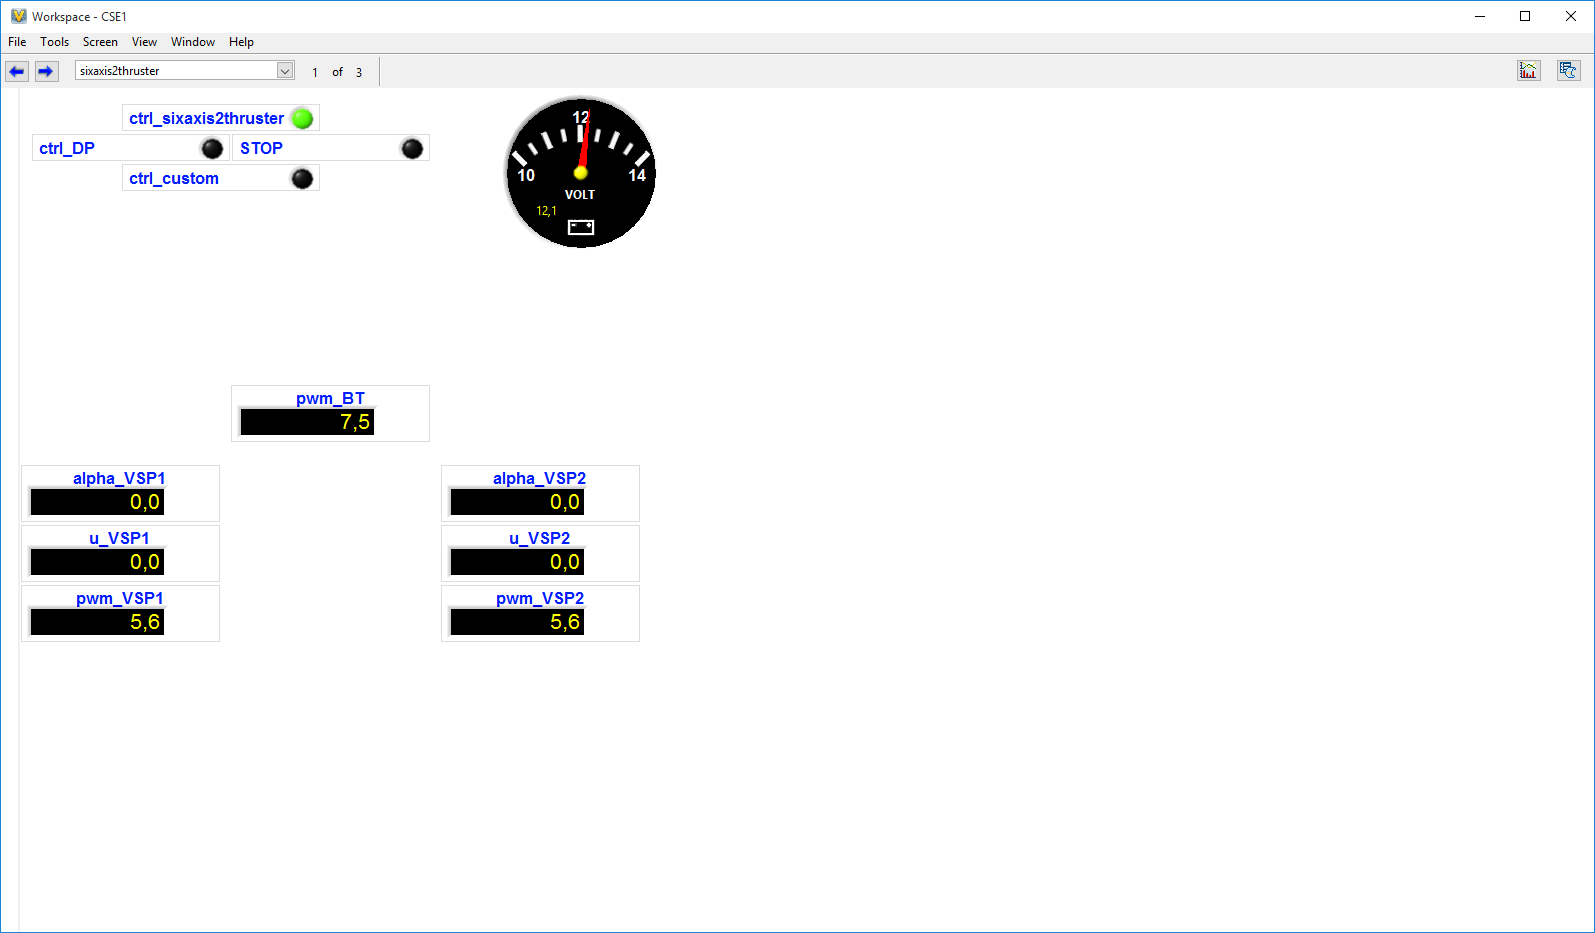
\includegraphics[width=\linewidth]{fig/CSE1_workspace_sixaxis2thruster.png}
	\caption{sixaxis2thruster workspace}
	\label{fig:workspace_sixaxis2thruster}
\end{figure}
In Figure \ref{fig:workspace_sixaxis2thruster} the workspace for sixaxis2thruster is illustrated. As the control mode is simply based on the sixaxis controller, the workspace only indicates the different variables on the vessel. 
\paragraph{ctrl\_DP}
\begin{figure}[htb!]
	\centering
	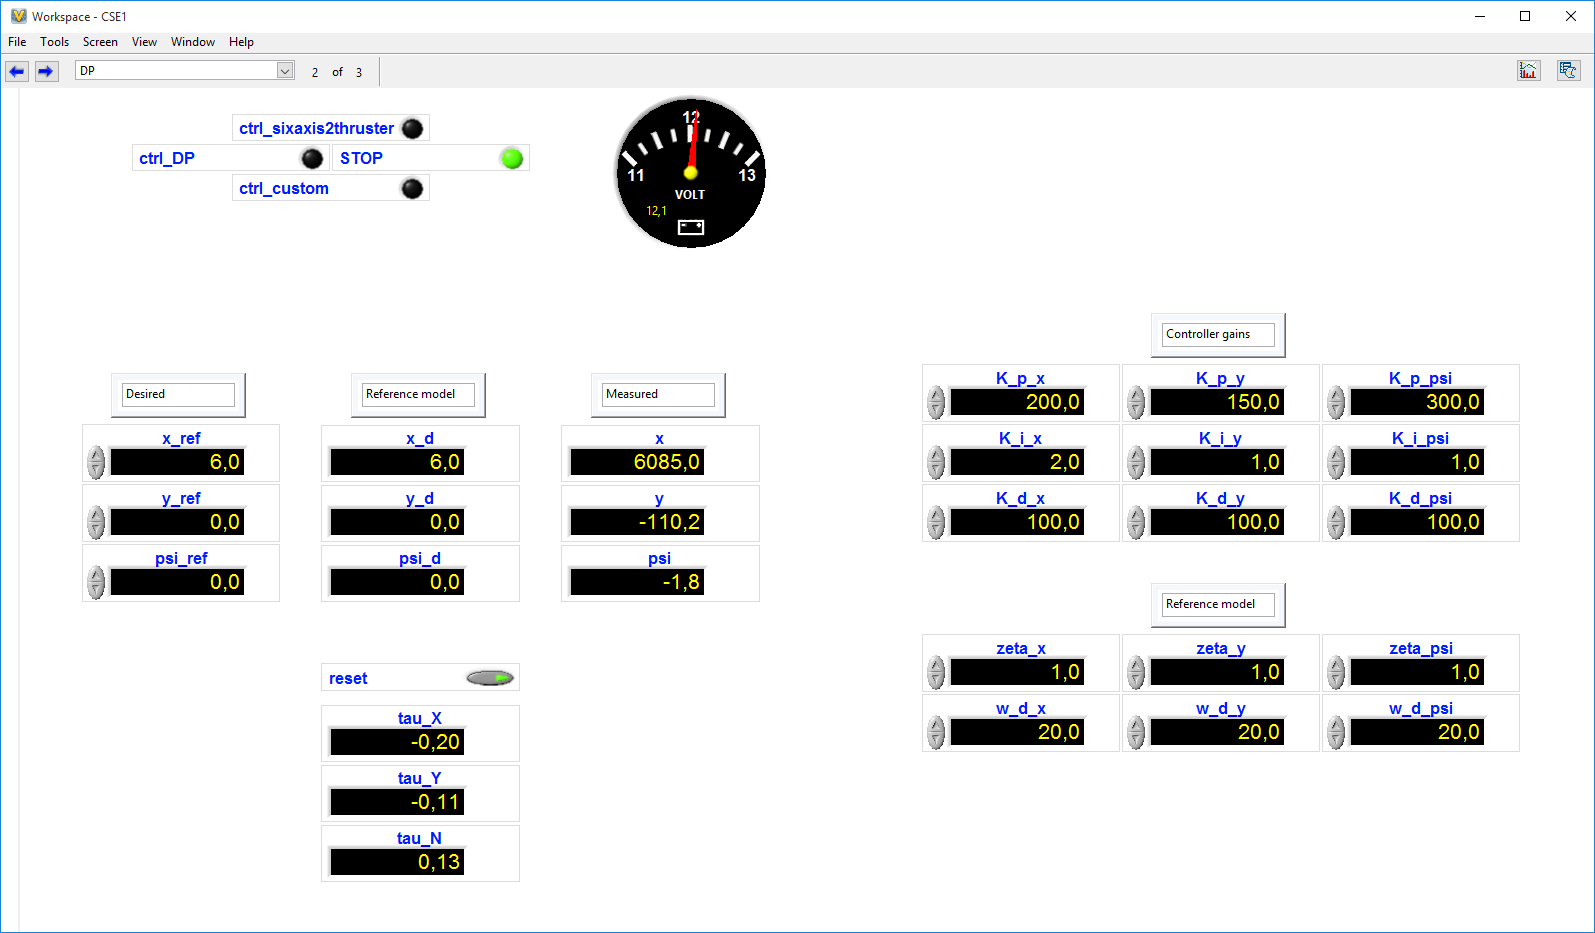
\includegraphics[width=\textwidth]{fig/CSE1_workspace_DP.png}
	\caption{DP workspace}
	\label{fig:workspace_DP}
\end{figure}
In Figure \ref{fig:workspace_DP} the workspace for the DP code is shown. Here, you define the set point for the reference model, and it's current position and orientation is given. On the right side, the model is tuned. There are some initial values, which provides a functional DP-system. 
\paragraph{ctrl\_custom}
\begin{figure}[htb!]
	\centering
	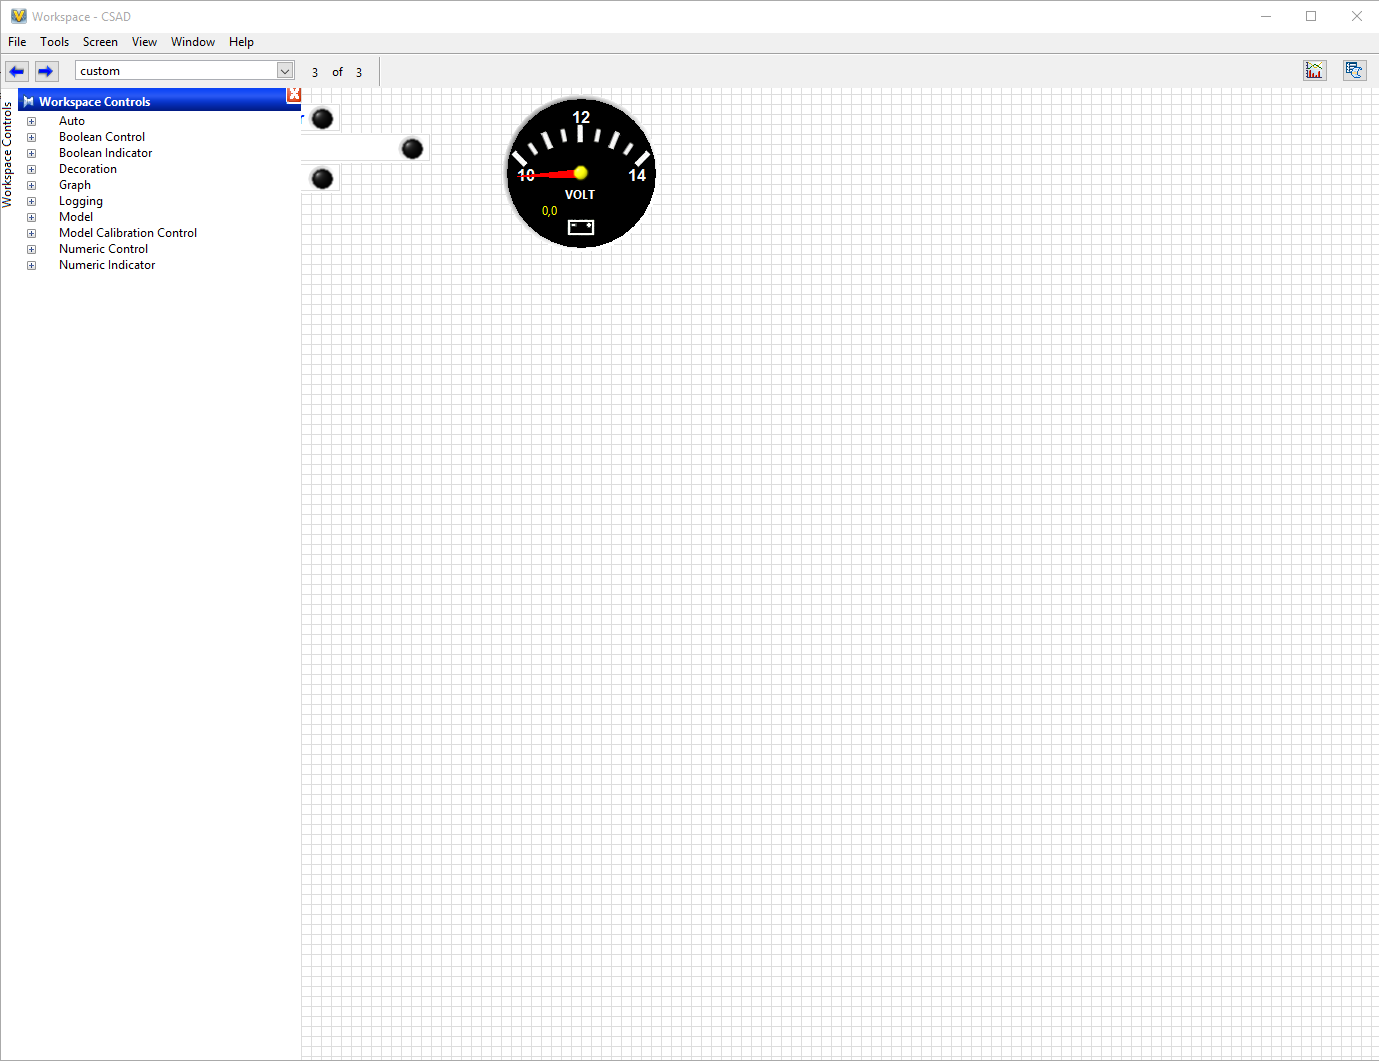
\includegraphics[width=\linewidth]{fig/CSAD_workspace_custom}
	\caption{custom workspace}
	\label{fig:workspace_custom}
\end{figure}
In Figure \ref{fig:workspace_custom} the workspace window for the customized control mode is illustrated. This is the one you should use when testing your control mode design. If you need more screens, press Screen -> Add Screen. To edit one screen, press Screen -> Edit Mode. On the left side(Workspace Controls), you can add different controls or indicators to monitor variables in the simulation model. Press 
\includegraphics{fig/magnifying_glass.png} and browse for the parameter you want to control/monitor, see Figure \ref{fig:workspace}. For example, real-time tuning of controller gains can be done by adding a Numeric Control->Meter and linking it to the variable. Use the scale option to enable higher precision when tuning. 
\begin{figure}[htb!]
	\centering
	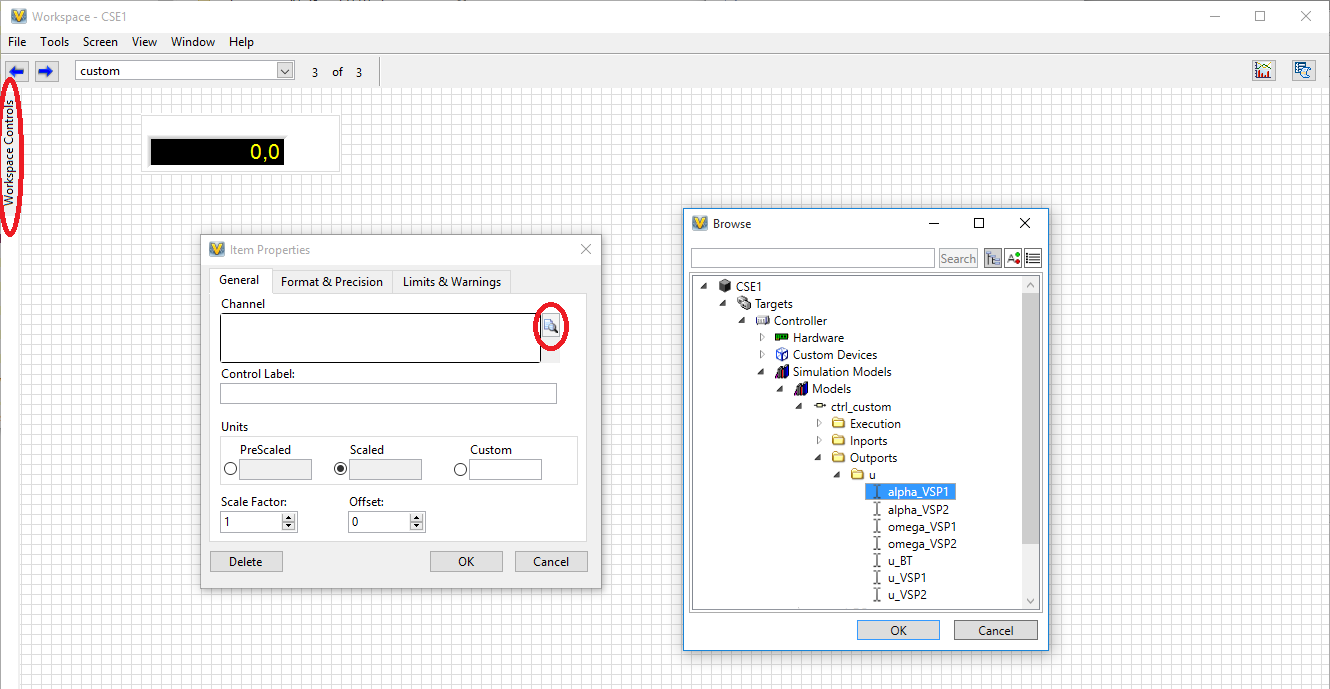
\includegraphics[scale=0.4]{fig/workspace_edit.png}
	\caption{Workspace window in Edit Mode}
	\label{fig:workspace}
\end{figure}
\chapter{Demolition}
When the experiments are finished, follow the procedure given here to shut down. 
\begin{enumerate}
	\item Switch to \textit{ctrl\_sixaxis2thruster}, and navigate CSE1 near the basin wall
	\item In the Project Explorer window, press to undeploy the code
	\item Disconnect the battery(negative first, then positive)
	\item Remove the battery, and set it to charge in the storage
	\item Lift CSE1 from the basin, and put it in its rack
	\item Leave the sixaxis controller in the vessel
	\item On the Qualisys computer, quit Qualisys Track Manager
	\item If you recorded any videos with the Camera System, export these videos to a memory stick, quit the software and turn of the TV-monitor
	\item Do a general clean up, bring all your personal belongings with you when you leave
\end{enumerate}